\vspace*{-2pt}
\section{Background}\label{sect:background}

\begin{figure}[tp]
	\centering
	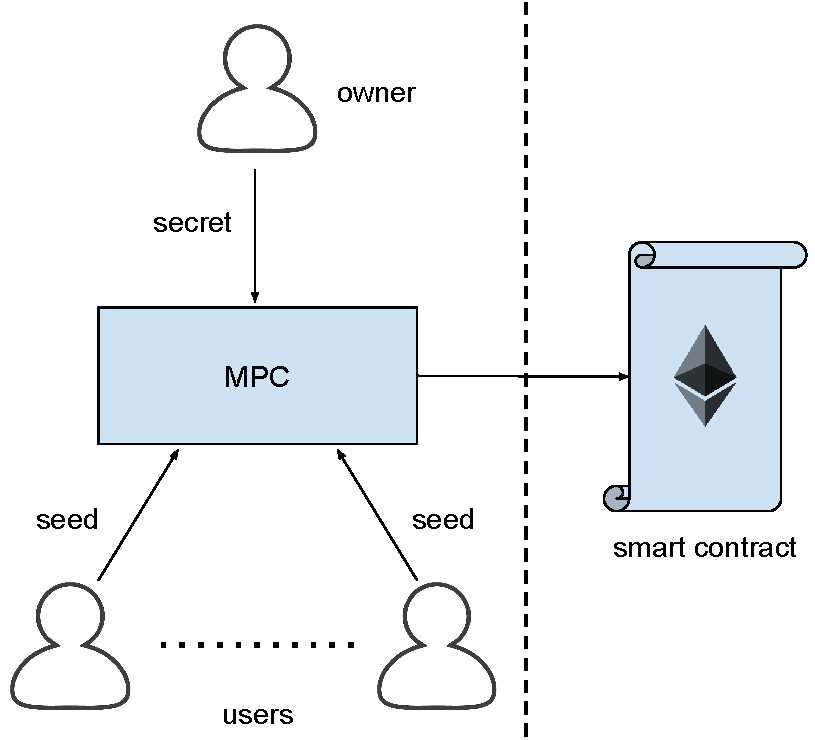
\includegraphics[width=0.75\textwidth]{fig/proposal}
	\vspace*{11pt}
	\caption{\name (\shortname) reference diagram}
	\label{fig:model}
\end{figure}



%This section illustrates the background concepts that will be used in the remainder of the chapter.

\paragraph*{Threshold Cryptography}

Threshold cryptography~\cite{Shamir:1979:SS:359168.359176} enables the owner of a secret to share it among a group of participants. 
In a \KofN threshold scheme, \N shares of the secret are created and, usually, one is given to each participant.\todo{Participants may get more than 1 share each, e.g., if someone is more reliable or has a higher reputation} 
To reconstruct the secret, at least \K different shares have to be combined.
Hence, the advantages of threshold cryptography are (i) distribution of trust,
%(at least \K participants are required to reconstruct the secret), 
and (ii) fault tolerance.
%(any subset of \N participants is sufficient).

\smallskip

\paragraph*{Secure Multi-Party Computation}

A {\em secure Multi-Party Computation (\em sMPC)} protocol~\cite{DBLP:journals/corr/abs-1804-03548,yao82} is a cryptographic protocol that allows multiple parties to jointly compute a function over their inputs while keeping them private.
%In sMPC, inputs are never visible to the other participants of the protocol, and the outputs of the functions can be made available to a subset of them. 
%After~\cite{yao82,yao86}, which firstly introduced the concept of MPC by computing a logic function between two parties, a lot of progress has been made~\cite{DBLP:journals/corr/abs-1804-03548}.
Current sMPC frameworks are able to execute binary or modular arithmetic algorithms computed among several parties (even with dishonest majority) by leveraging {\em semi-homomorphic encryption}~\cite{spdz,keller2018overdrive} and {\em oblivious transfer}~\cite{mascot,rabin2005exchange}.

\smallskip

\paragraph*{Smart contracts}

A blockchain is an append-only list of blocks linked together via cryptographic properties. The blocks in the blockchain are non-mutable and are used to keep a permanent history of transactions.
Smart contracts~\cite{szabo1997formalizing} are programming frameworks built on top of blockchains.
A smart contract permits to program tamper-proof protocols whose outcome is verifiable by the whole network.
%
%Indeed, any piece of data stored in a smart contract can be verified by any peer of the network, and read by anyone.
%
%Several blockchain-based architectures have been proposed to overcome this limitation. Enigma~\cite{enigma} by Zyskind et al. and Hawk~\cite{hawk} by Kosba et al. address the issue by leveraging Multi-Party Computation~\cite{DBLP:journals/corr/abs-1804-03548,yao82} to allow several actors to execute functions over secret inputs without getting to know the underlying plaintext.
%%
%Yet, these architectures can not be used in the TL setting, as they require the data holder to actively take part in the computation.
We rely on smart contracts to pay incentives, trigger penalties, and in general to enforce the correct execution of our scheme without the need of a trusted party.
Specifically, our approach makes use of the {\em time} and {\em hash} primitives, which are used to conditionally execute actions based on time and submitted data, respectively.
We remark that the {\em time} primitive differs from TL in that it does not keep any data confidential.

\smallskip

\paragraph*{Rational adversaries}

A malicious adversary~\cite{Hazay10anote} is someone who is willing to perform any action to attack a protocol. A rational adversary~\cite{Groce2012}, instead, subverts the protocol only if it is economically convenient.
%has a stake in the protocol success, and therefore tries to violate the protocol, such as colluding with other parties, only when the expected outcome is greater than the one obtained by complying with the rules. 
Modeling the participants as rational enables the use of game theory concepts to analyze cryptographic protocols~\cite{Asharov2016,raap,Provi07summaryreport}.
%
%Rational cryptography~\cite{raap}, \cite{Provi07summaryreport} analyzes cryptographic protocols, run by rational adversaries, by the application of game theory methodology.
%It has been shown that game theoretic concepts can be used to capture the cryptographic notion of security.
\shortname models all the participants as rational, and it does not rely on any trust or honesty assumption on them.
